\documentclass[12pt, letterpaper]{article}
\usepackage{graphicx}
\graphicspath{ {images/} }

\title{CometTS (Comet Time Series (CometTS) Visualizer)} 
\author{Dante Lozano-Perez}\thanks{Mun Summer2020 CMSC6950}
\date{\today}

\begin{document}
\maketitle
\section{Introduction}
Comet Time Series is a python tool with the objective of creating different time series from a region of interest. this program uses images and CSV files to create a time series analisis.

\section{Content}

The program demo, is creating a time series analisis of San Juan, Puerto Rico. This analisis is made from the VIIRS images from the satelite and create a forecast using ARIMA models.


\section{Graphs}
\begin{figure}
    \centering
    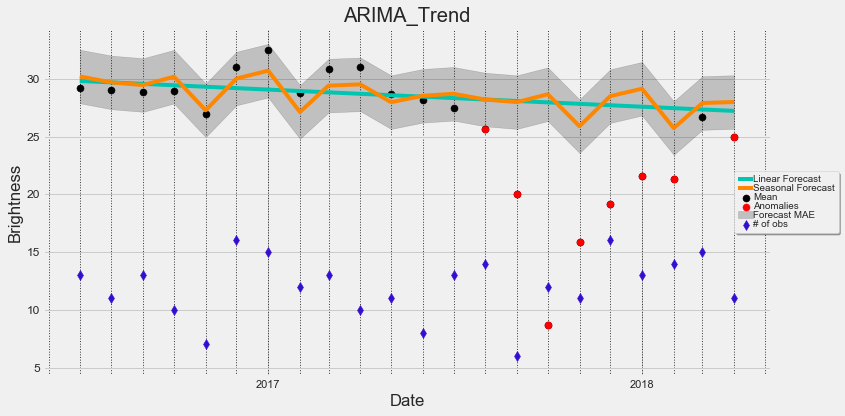
\includegraphics[width=0.5\textwidth]{ARIMA.png}
\end{figure}

\section{Conclusion}
In Conclusion, We can see that with this program, it is easy to observe the changes that the place, in this case San Juan, Puerto Rico, has been throughout the time and also create a quick forecast of the area.

\end{document}